\pdfoutput=1
\documentclass[11pt]{article}
\usepackage[margin=1in]{geometry}
\usepackage{amsmath,amssymb,amsthm,booktabs,array}
\usepackage[shortlabels]{enumitem}
\usepackage[hidelinks]{hyperref}
\usepackage{algorithm}
\usepackage[noend]{algpseudocode}
\usepackage{tikz}
\usetikzlibrary{arrows.meta,backgrounds,calc,positioning,fit}
\tikzset{
  v/.style={circle,draw,fill=white,inner sep=0pt,minimum size=6pt,line width=0.6pt},
  d/.style={circle,fill=black,inner sep=0pt,minimum size=4.5pt},
  e/.style={line width=0.6pt},
  faint/.style={line width=0.5pt,black!30},
  arc/.style={line width=0.6pt,-{Stealth[length=4.5pt]}},
  lab/.style={font=\scriptsize},
  box/.style={draw,rounded corners=2pt,line width=0.6pt,align=center,font=\footnotesize,inner sep=4pt,minimum height=20pt},
  tool/.style={box,fill=black!6},
  main/.style={box,line width=1.1pt},
}


\setlist{itemsep=1pt,topsep=3pt}

\newtheorem{theorem}{Theorem}[section]
\newtheorem{lemma}[theorem]{Lemma}
\newtheorem{corollary}[theorem]{Corollary}
\theoremstyle{definition}
\newtheorem{definition}[theorem]{Definition}
\theoremstyle{remark}
\newtheorem{remark}[theorem]{Remark}

\newcommand{\Ot}{\tilde O}
\newcommand{\AlgNest}{\textsc{NestedSearch}}
\newcommand{\inner}[2]{\langle #1,#2\rangle}

\title{Quantum Query Complexity of the Maximum\\ of a Totally Monotone Matrix}
\hypersetup{pdftitle={Quantum Query Complexity of the Maximum of a Totally Monotone Matrix},pdfauthor={Sebastian Senge}}
\author{Sebastian Senge\\ Independent Researcher}
\date{}

\begin{document}
\maketitle

\begin{abstract}
We study the number of quantum queries needed to find the largest entry of a totally monotone $r\times c$ matrix, where a query returns one entry. Write $n=\max(r,c)$. Classically $\Theta(n)$ queries are necessary and sufficient. Our results are these:
\begin{itemize}[leftmargin=1.5em]
\item Deciding whether the maximum is at least a given value takes $O(\sqrt n\log n)$ queries.
\item The maximum and its position take $O(\sqrt n\log^3 n\log\log n)$ queries, with no dependence on the range of the entries.
\item An explicit nested quantum search takes $\sqrt n\cdot 2^{O(\sqrt{\log n\log\log n})}$ queries, and $\Ot(n^{3/4})$ queries in its simplest form.
\item At least $\Omega(\sqrt n)$ queries are necessary, already for matrices satisfying the reverse quadrangle inequality.
\item The diameter of a strictly convex polygon with $n$ vertices takes $\Ot(\sqrt n)$ queries, and $\Omega(\sqrt n)$ queries are necessary.
\end{itemize}
These are query bounds on a noiseless model. The two sharpest upper bounds go through the adversary bound and give no bound on gates or time.
\end{abstract}

\section{Introduction}

A matrix $M$ with entries in a totally ordered set is \emph{totally monotone} if for all rows $i<i'$ and columns $j<j'$,
\[
M[i,j]<M[i,j'] \implies M[i',j]<M[i',j'].
\]
This class contains every matrix with the \emph{reverse quadrangle inequality} $M[i,j]+M[i',j']\ge M[i,j']+M[i',j]$. Such matrices are a standard tool in computational geometry and dynamic programming, and the algorithm of~\cite{AKMSW87} finds all row maxima of an $r\times c$ totally monotone matrix with $O(r+c)$ entry reads.

Here a query $(i,j)$ returns $M[i,j]$, and the task is to find the largest entry of $M$. Quantum maximum finding~\cite{DH96} over all entries costs $\Theta(\sqrt{rc})$ queries, which is $\Theta(n)$ on square matrices, so a quantum gain has to use the structure. We show that the structure gives a quadratic gain.

\begin{table}[h]
\centering
\small
\renewcommand{\arraystretch}{1.25}
\begin{tabular}{@{}lllll@{}}
\toprule
Problem & Previous best bound & Our bound & Lower bound & Section\\
\midrule
Is $\max M\ge\theta$? & $O(n)$ \cite{AKMSW87} & $O(\sqrt n\log n)$ & $\Omega(\sqrt n)$ & \ref{sec:adv}\\
$\max M$ and its position & $O(n)$ \cite{AKMSW87} & $O(\sqrt n\log^3 n\log\log n)$ & $\Omega(\sqrt n)$ & \ref{sec:adv}\\
Same, explicit search & $O(n)$ \cite{AKMSW87} & $\sqrt n\cdot 2^{O(\sqrt{\log n\log\log n})}$ & $\Omega(\sqrt n)$ & \ref{sec:nested}\\
Polygon diameter, decision & $\Ot(n^{3/4})$ \cite{Zaj23} & $O(\sqrt n\log^{3/2} n)$ & $\Omega(\sqrt n)$ & \ref{sec:polygon}\\
Polygon diameter, value & $\Ot(n^{3/4})$ \cite{Zaj23} & $O(\sqrt n\log^{7/2} n\log\log n)$ & $\Omega(\sqrt n)$ & \ref{sec:polygon}\\
\bottomrule
\end{tabular}
\caption{Quantum query bounds, with $n=\max(r,c)$ for matrices and $n$ vertices for polygons. The polygon baseline \cite{Zaj23} holds for the diameter of a general point set, and it is a bound on time as well as on queries. All classical randomized algorithms need $\Omega(n)$ queries on these problems.}
\label{tab:results}
\end{table}

To our knowledge there is no earlier quantum result on totally monotone matrix search, or on the diameter of a convex polygon. The closest result known to us is the bound of~\cite{Zaj23} for a general point set, on which the structure used here is not available.

\paragraph{Techniques.} Computing the row maximum of a middle row splits a matrix into two parts with windows of columns whose widths sum to $c+1$. A direct nesting of quantum searches pays a polylogarithmic overhead at every level of the recursion, which leaves a subpolynomial factor. In Section~\ref{sec:adv} we run the same recursion on filtered factorization norms~\cite{LMRSS11}, which compose with no such loss, and we obtain two composition lemmas for this purpose.

\paragraph{Scope.} All bounds count queries on a noiseless model. The algorithm behind the bounds of Section~\ref{sec:adv} exists through the general theorem of~\cite{LMRSS11}, and it is not efficient in gates as stated. The algorithm of Section~\ref{sec:nested} is an explicit composition of quantum searches. Section~\ref{sec:lean} states which parts are formalized in Lean. The other parts are claims with the proofs given here.

\section{Preliminaries}

Let $M$ be totally monotone, and let $p(i)$ be the leftmost column in which row $i$ attains its maximum.

\begin{lemma}\label{lem:mono}
The function $p$ is nondecreasing.
\end{lemma}
\begin{proof}
Let $i<i'$ and suppose $j':=p(i')<j:=p(i)$. By the choice of $j$, $M[i,j']<M[i,j]$, since $j'<j$ and $j$ is the leftmost maximum of row $i$. Total monotonicity gives $M[i',j']<M[i',j]$, a contradiction with $j'$ being a maximum of row $i'$.
\end{proof}

Leftmost maxima matter here. The matrix with rows $(1,1)$ and $(2,0)$ is totally monotone, and taking column $2$ for the first row would hide the maximum of the second row. So every maximum finding below runs on the pair of the value and the negated column index.

\paragraph{Quantum primitives.} A maximum over $N$ items costs at most $\kappa\sqrt N$ queries with bounded error, for a constant $\kappa$~\cite{DH96}. If item $i$ has a known cost bound $t_i$, then a search over the items costs $\Ot(\sqrt{\sum_i t_i^2})$ queries~\cite{Amb10}.

\section{Lower bounds}\label{sec:lower}

\begin{theorem}\label{thm:lower}
For $h\in\{0,1\}^n$ let $M_h[i,j]=-(i-j)^2$ for $i\ne j$ and $M_h[i,i]=h_i$. Then $M_h$ satisfies the reverse quadrangle inequality, and its maximum is the OR of $h$. So computing the maximum needs $\Omega(\sqrt n)$ quantum queries and $\Omega(n)$ classical randomized queries.
\end{theorem}
\begin{proof}
It suffices to check adjacent $2\times 2$ blocks. Let $D=M[i,j]+M[i+1,j+1]-M[i,j+1]-M[i+1,j]$. The matrix with $h=0$ has $D=2$. Raising a diagonal entry by $h_i\le 1$ raises $D$ by $h_i$ on a block with that entry on its main diagonal and lowers $D$ by $h_i$ on a block with it on the other diagonal. A block contains at most two diagonal entries, and when it contains two, both lie on its main diagonal. So $D\ge 1$ in every case.
\end{proof}

\section{An explicit nested search}\label{sec:nested}

\begin{figure}[ht]
\centering
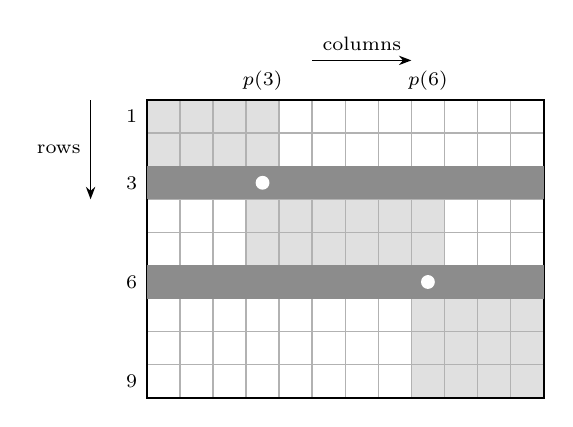
\begin{tikzpicture}[x=0.42cm,y=-0.42cm]
  % blocks left after the row maxima of rows 3 and 6
  \fill[black!12] (0,0) rectangle (4,2);
  \fill[black!12] (3,3) rectangle (9,5);
  \fill[black!12] (8,6) rectangle (12,9);
  \foreach \x in {1,...,11} \draw[faint] (\x,0) -- (\x,9);
  \foreach \y in {1,...,8} \draw[faint] (0,\y) -- (12,\y);
  \draw[e] (0,0) rectangle (12,9);
  \fill[black!45] (0,2) rectangle (12,3);
  \fill[black!45] (0,5) rectangle (12,6);
  \node[d,white,minimum size=5pt] at (3.5,2.5) {};
  \node[d,white,minimum size=5pt] at (8.5,5.5) {};
  \foreach \i/\l in {0.5/1,2.5/3,5.5/6,8.5/9} \node[lab,left] at (0,\i) {\l};
  \node[lab,above] at (3.5,0) {$p(3)$};
  \node[lab,above] at (8.5,0) {$p(6)$};
  \draw[arc] (-1.7,0) -- node[lab,left] {rows} (-1.7,3);
  \draw[arc] (5,-1.2) -- node[lab,above] {columns} (8,-1.2);
\end{tikzpicture}

\caption{Depth one on a $9\times 12$ matrix with $k=2$ chosen rows. By Lemma~\ref{lem:mono}, the maxima of the remaining rows lie in the shaded blocks, whose column widths sum to at most $c+k$.}
\label{fig:windows}
\end{figure}

At depth $0$, search all $rc$ cells by maximum finding, at $\kappa\sqrt{rc}$ queries. At depth $d$ the algorithm is as follows.

\begin{algorithm}[h]
\caption{\AlgNest$(d)$ on rows $s,\dots,t$ and columns $l,\dots,u$}
\begin{algorithmic}[1]
\State $r\gets t-s+1$, $k\gets\lceil r^{1/(d+1)}\rceil$; choose $k$ evenly spaced rows
\State compute the leftmost maxima of the chosen rows in bisection order: find $p$ for the middle chosen row on the current window, then continue above it with the window $[l,p]$ and below it with the window $[p,u]$
\State this leaves $k+1$ blocks of rows with windows of widths $c_i$
\State \Return the largest of the row maxima found and the results of \AlgNest$(d-1)$ on the blocks, using a quantum search over the blocks
\end{algorithmic}
\end{algorithm}

\paragraph{Cost of a level.} At level $j$ of the bisection the windows of the $2^j$ rows have total width at most $c+2^j$. So that level costs at most $\kappa\sqrt{2^j(c+2^j)}$, since $\sum_i\sqrt{x_i}\le\sqrt{m\sum_i x_i}$ for $m$ terms. The sum over the levels is $O(\sqrt{k(c+k)})$, and the windows of the blocks satisfy $\sum_i c_i\le c+k$.

\paragraph{The overhead $C$.} Let the search over the blocks cost $C\sqrt{\sum_i t_i^2}$ queries, where the $t_i$ are known cost bounds. The factor $C$ is polylogarithmic in $n$, and it includes three things beyond~\cite{Amb06,Amb10}. Inner runs have bounded error and need error reduction and uncomputation at each level. All $k$ row maxima must be right, which adds a factor $\log k$ to the first term. And a maximum over the blocks needs more than a search for one marked item, which the prefix bisection of Section~\ref{sec:adv} provides at polylogarithmic cost.

\begin{theorem}\label{thm:nested}
The cost at depth $d$ is $T_d(r,c)\le O(C^d)\sqrt{r+c}\cdot r^{1/(2d+2)}$. So depth $1$ gives $\Ot(n^{3/4})$, and depth $d\approx\sqrt{\log n/\log C}$ gives $\sqrt n\cdot 2^{O(\sqrt{\log n\log\log n})}$ queries.
\end{theorem}
\begin{proof}
Correctness follows from Lemma~\ref{lem:mono}: each row has its leftmost maximum in its window, so the windows contain a largest entry.

For the cost, use induction with $a_d=1/(2d+2)$, where $a_0=1/2$ matches $T_0=\kappa\sqrt{rc}$. Up to constant factors,
\[
T_d(r,c)\le\sqrt{k(c+k)}+C\sqrt{\sum_i T_{d-1}(r/k,c_i)^2}\le\sqrt{k(r+c)}+C^d\sqrt{r+c}\,(r/k)^{a_{d-1}}.
\]
With $k=r^{1/(d+1)}$ the first term is $\sqrt{r+c}\;r^{1/(2d+2)}$, and the second has exponent $(1-\frac1{d+1})\cdot\frac1{2d}=\frac1{2d+2}$.
\end{proof}

At depth $1$ there is no nesting: compute about $\sqrt r$ row maxima, and then run one maximum finding over the $O(n^{3/2})$ remaining cells.

\section{Removing the overhead}\label{sec:adv}

Nesting pays $C$ at each level. The filtered factorization norm has no such loss.

\begin{definition}[\cite{LMRSS11}]
Let $D$ be a set of inputs, and let $\Delta_j[x,y]=1$ if $x_j\ne y_j$ and $0$ otherwise. For a matrix $A$ on $D\times D$,
\[
\gamma_2(A\mid\Delta)=\min\ \max\Bigl(\max_x\sum_j\|u_{xj}\|^2,\ \max_y\sum_j\|v_{yj}\|^2\Bigr)\quad\text{where}\quad A[x,y]=\sum_j\Delta_j[x,y]\inner{u_{xj}}{v_{yj}}.
\]
For $f$ on $D$ let $F_f[x,y]=1$ if $f(x)=f(y)$ and $0$ otherwise, and put $\gamma(f)=\gamma_2(J-F_f\mid\Delta)$, where $J$ is the all-ones matrix.
\end{definition}

By~\cite{LMRSS11}, the query complexity $Q$ and the general adversary bound satisfy $Q(f)=\Theta(\mathrm{Adv}^\pm(f))$ and $\mathrm{Adv}^\pm(f)\le\gamma(f)\le 2\,\mathrm{Adv}^\pm(f)$. So $Q(f)=O(\gamma(f))$ and $\gamma(f)=O(Q(f))$ for every $f$.

\begin{lemma}[Sequential composition]\label{lem:seq}
Let $A:D\to E$, and for each $a\in E$ let $G_a$ be a function on $D_a=A^{-1}(a)$. Let $h(x)=G_{A(x)}(x)$. Then $\gamma(h)\le 2\gamma(A)+\max_a\gamma(G_a)$.
\end{lemma}
\begin{proof}
Let $\alpha(x,y)=1$ if $A(x)\ne A(y)$ and $\beta(x,y)=1$ if $h(x)\ne h(y)$, with both $0$ otherwise. Then
\[
\beta=\alpha+(1-\alpha)\beta-(1-\beta)\alpha,
\]
since the right side expands to $\alpha+\beta-\alpha\beta-\alpha+\alpha\beta$. The first term is $J-F_A$. The second term, on a pair with $A(x)=A(y)=a$, is $J-F_{G_a}$, and it vanishes on other pairs. Tagging vectors with $A(x)$, so that vectors of different classes are orthogonal, gives a factorization of cost $\max_a\gamma(G_a)$. The third term is $J-F_A$ restricted to pairs with $h(x)=h(y)$. Tagging the factorization of $J-F_A$ with $h(x)$ gives it at cost $\gamma(A)$. Filtered factorizations add by direct sum, and their costs add.
\end{proof}

\begin{lemma}[OR]\label{lem:or}
For binary functions $g_1,\dots,g_k$ on $D$ and $\mathrm{OR}(x)=\bigvee_i g_i(x)$, we have $\gamma(\mathrm{OR})\le\sqrt{\sum_i\gamma(g_i)^2}$.
\end{lemma}
\begin{proof}
Let $a_i=\gamma(g_i)$ and $S=\sqrt{\sum_i a_i^2}$, and let $(u^i,v^i)$ factor $J-F_{g_i}$ with squared norm at most $a_i$ on each input. If some $a_i=0$ then $g_i$ is constant on $D$: the constant $1$ makes OR constant, and the constant $0$ can be dropped. So take all $a_i>0$. If $\mathrm{OR}(x)=0$, put
\[
U_x=\bigoplus_i\sqrt{a_i}\,u^i_x,\qquad W_x=\bigoplus_i\sqrt{a_i}\,v^i_x,
\]
both of squared norm at most $\sum_i a_i^2=S^2$. If $\mathrm{OR}(y)=1$, fix $i=i(y)$ with $g_i(y)=1$, and put $T_y=a_i^{-1/2}u^i_y$ and $V_y=a_i^{-1/2}v^i_y$ on block $i$ and $0$ elsewhere, both of squared norm at most $1$. For $\mathrm{OR}(x)=0$ and $\mathrm{OR}(y)=1$ the function $g_{i(y)}$ differs on $x$ and $y$, so $\sum_j\Delta_j\inner{U_{xj}}{V_{yj}}=1$ and $\sum_j\Delta_j\inner{T_{yj}}{W_{xj}}=1$. Now use two orthogonal slots:
\begin{align*}
\mathrm{OR}(x)=0:&\quad L_x=S^{-1/2}(U_x,0),\quad R_x=S^{-1/2}(0,W_x),\\
\mathrm{OR}(y)=1:&\quad L_y=S^{1/2}(0,T_y),\quad\ \ R_y=S^{1/2}(V_y,0).
\end{align*}
Pairs with different OR give $1$ in both orders. Pairs with the same OR give $0$, since their nonzero slots differ. All squared norms are at most $S$.
\end{proof}

\begin{theorem}\label{thm:decide}
On totally monotone $r\times c$ matrices and for fixed $\theta$, the function $F(M)=[\max M\ge\theta]$ has $\gamma(F)\le(2\kappa+1)\lceil\log_2(r+1)\rceil\sqrt{r+c}$. So $Q(F)=O(\sqrt n\log n)$.
\end{theorem}
\begin{proof}
Fix rows $s,\dots,t$ and columns $l,\dots,u$, with $r=t-s+1$ and $c=u-l+1$. Let $D[s,t,l,u]$ be the totally monotone inputs whose leftmost maxima on these rows lie in $[l,u]$, and let $F[s,t,l,u]$ be the statement that some entry in these rows and columns is at least $\theta$. On this domain that is the same as some row maximum being at least $\theta$. Let $\Gamma(r,c)$ be the largest $\gamma$ over such domains, with $\Gamma(0,c)=0$.

For $r=1$ this is an OR of $c$ bits, and each bit has $\gamma=1$, so $\Gamma(1,c)\le\sqrt c$ by Lemma~\ref{lem:or}.

For the step let $m=\lfloor(s+t)/2\rfloor$ and $A(x)=p(m)$. Maximum finding on $[l,u]$ computes $A$, so $\gamma(A)\le\kappa\sqrt c$, where $\kappa$ now also includes the constant of $\gamma=O(Q)$. On $A^{-1}(p)$, Lemma~\ref{lem:mono} gives the domain $D[s,m-1,l,p]\cap D[m+1,t,p,u]$, and on it
\[
F[s,t,l,u]=[x_{m,p}\ge\theta]\vee F[s,m-1,l,p]\vee F[m+1,t,p,u].
\]
Restriction to a subdomain does not raise $\gamma$. Lemmas~\ref{lem:seq} and~\ref{lem:or} give, with $r_1+r_2=r-1$ and $c_1+c_2=c+1$,
\[
\Gamma(r,c)\le 2\kappa\sqrt c+\sqrt{1+\Gamma(r_1,c_1)^2+\Gamma(r_2,c_2)^2}.
\]
Let $\ell(r)=\lceil\log_2(r+1)\rceil$ and $a=2\kappa+1$. Assume $\Gamma(r_i,c_i)\le a\,\ell(r_i)\sqrt{r_i+c_i}$, where $\ell(r_i)\le\ell(r)-1$. Since $(r_1+c_1)+(r_2+c_2)=r+c$, the square root is at most $1+a(\ell(r)-1)\sqrt{r+c}$. So $\Gamma(r,c)\le 2\kappa\sqrt c+1+a(\ell(r)-1)\sqrt{r+c}\le a\,\ell(r)\sqrt{r+c}$.
\end{proof}

\begin{corollary}\label{cor:max}
For any range of the entries, the maximum of a totally monotone matrix and its position take $O(\sqrt n\log^3 n\log\log n)$ queries.
\end{corollary}
\begin{proof}
Deleting rows keeps total monotonicity, so the proof of Theorem~\ref{thm:decide} applies to any subset of rows and to the strict test ``some entry exceeds $\theta$''. Fix a random order of the rows, and let $S$ be the rows with a maximum above the current $\theta$. Bisect on prefixes of the order with the decision, with its error reduced by a factor $O(\log\log n)$. This gives the first row of $S$ in the order, which is uniform in $S$, using $O(\log n)$ decisions. Read the maximum of that row by maximum finding at $O(\sqrt c)$ queries, and set $\theta$ to it. In expectation $S$ halves, so $O(\log r)$ rounds suffice.
\end{proof}

\begin{remark}
By~\cite{LMRSS11}, any factorization gives a query algorithm built from reflections, so the algorithm exists and uses $O(\gamma)$ queries, but no bound on time follows. The recursion could be run by subroutine composition~\cite{Jef22} or transducers~\cite{BJY23}. We have not worked out either form.
\end{remark}

\section{Diameter of a convex polygon}\label{sec:polygon}

The input is an array with the vertices $v_0,\dots,v_{n-1}$ of a strictly convex polygon in counterclockwise order, and a query returns one vertex. The task is to find the largest distance between two vertices.

\begin{lemma}\label{lem:arc}
Let $a_1,\dots,a_s$ and $b_1,\dots,b_t$ be two arcs of consecutive vertices, disjoint, in this order around the polygon. Then $M[i,j]=|a_ib_j|$ satisfies the reverse quadrangle inequality, and the matrix of squared distances is totally monotone.
\end{lemma}
\begin{proof}
For $i<i'$ and $j<j'$, the segments $a_ib_j$ and $a_{i'}b_{j'}$ are the diagonals of a convex quadrilateral, so they cross at a point $P$. By the triangle inequality,
\[
|a_ib_j|+|a_{i'}b_{j'}|=|a_iP|+|Pb_j|+|a_{i'}P|+|Pb_{j'}|\ge|a_ib_{j'}|+|a_{i'}b_j|.
\]
Squares compare the same way as distances within a row, so the squared matrix is totally monotone, and it has integer entries on integer coordinates.
\end{proof}

\begin{theorem}\label{thm:polygon}
Deciding whether the diameter is at least a given value takes $O(\sqrt n\log^{3/2}n)$ queries, and the diameter itself takes $O(\sqrt n\log^{7/2}n\log\log n)$ queries. At least $\Omega(\sqrt n)$ quantum and $\Omega(n)$ classical randomized queries are necessary.
\end{theorem}
\begin{proof}
Halve the sequence of vertices recursively. Every pair is separated at exactly one node of the recursion, where it appears in a matrix for two arcs of sizes $s+t=n/2^\ell$, and there are $2^\ell$ such matrices at level $\ell$. One matrix query is at most four vertex queries, with uncomputation, so by Theorem~\ref{thm:decide} and $\gamma=O(Q)$ each matrix has $\gamma\le O(\log n)\sqrt{n/2^\ell}$ in the vertex model. Lemma~\ref{lem:or} over all matrices gives the squared cost $O(\log^2 n)\sum_\ell 2^\ell\cdot n/2^\ell=O(n\log^3 n)$.

For the value, run the prefix bisection of Corollary~\ref{cor:max} on the vertices. A prefix restricts each matrix to the pairs with an endpoint in the prefix, which is two totally monotone submatrices at the same cost bound. When the bisection returns a vertex, read its farthest vertex by maximum finding at $O(\sqrt n)$ queries.

For the lower bounds, take $n/2$ antipodal pairs of rational points on a circle of radius $R$. These points are in strictly convex position, the antipodal pairs have distance $2R$, and no other pair reaches it. Take one vertex $v$ from each pair and move it to $(1+\varepsilon)v$ if its bit is $1$. For small $\varepsilon$ this keeps strict convexity, which is an open condition on finitely many points, and a moved vertex has distance $(2+\varepsilon)R$ from its antipode. So the decision whether the diameter exceeds $2R$ computes the OR of $n/2$ bits.
\end{proof}

\section{Simulation and circuits}\label{sec:sim}

The repository has simulation scripts, some of which sample each search from the exact outcome law of quantum search with a budget per search, and a circuit test.
\begin{itemize}[leftmargin=1.5em]
\item The nested search agrees with brute force on $1500$ runs, and the polygon routine agrees with brute force and with rotating calipers on $144$ runs.
\item At depth $1$ and $n=2048$, the count is $35\,n^{3/4}$ to $51\,n^{3/4}$ oracle applications at a budget of $16$ per search, with no wrong answers at budget $16$ or more.
\item The classical algorithm of~\cite{AKMSW87} reads $3.5n$ to $5n$ entries in the same runs, so depth $1$ passes it only for $n$ of order $10^4$, by extrapolation.
\item With every search a circuit in Qiskit, on at most $8$ qubits, $30$ runs give no wrong answer.
\item The recursion of Theorem~\ref{thm:decide}, evaluated on single inputs with a base cost of one, gives $1.96$ to $2.01$ times $\sqrt n\log_2 n$ for $n$ from $64$ to $4096$.
\end{itemize}
These runs test the constructions. The constant $\kappa$ in Theorem~\ref{thm:decide} is not known, so the logarithmic factors there say nothing at practical sizes.

\section{Formal verification}\label{sec:lean}

The Lean files in the repository build with no \texttt{sorry}, and \texttt{\#print axioms} reports only the standard axioms.

\paragraph{Proved outright.} Total monotonicity from the reverse quadrangle inequality, Lemma~\ref{lem:mono} and the windows, the hard family of Theorem~\ref{thm:lower}, the classical skeleton of the algorithm of Section~\ref{sec:nested} with its width sums, Lemma~\ref{lem:arc}, Lemmas~\ref{lem:seq} and~\ref{lem:or}, the recurrence of Theorem~\ref{thm:decide} on $\gamma$, the round count of Corollary~\ref{cor:max}, and the arithmetic of Theorem~\ref{thm:nested}.

\paragraph{Stated as hypotheses.} The two theorems of~\cite{LMRSS11} quoted in Section~\ref{sec:adv}, the cost of maximum finding, and the recursion for $T_d$ in the arithmetic of Theorem~\ref{thm:nested}. With these, Theorem~\ref{thm:decide} holds in Lean as a bound on $Q$, with a constant independent of $r$, $c$, the alphabet and $\theta$.

\paragraph{Not formalized.} The definitions of $Q$ and of the adversary bound are not unfolded by any proof, so their match with the literature rests on reading them. Also not formalized are Corollary~\ref{cor:max} as a bound on $Q$ (error reduction, adaptive composition and the step from mean to worst case), the quantum algorithm and the variable-time search of Theorem~\ref{thm:nested}, the OR lower bounds of Theorem~\ref{thm:lower}, and Theorem~\ref{thm:polygon} apart from Lemma~\ref{lem:arc}.

\section{Open questions}

\begin{itemize}[leftmargin=1.5em]
\item An explicit algorithm with $\Ot(\sqrt n)$ queries and a matching bound on gates.
\item The exact power of the logarithm. Between $\Omega(\sqrt n)$ and $O(\sqrt n\log n)$ the decision problem is open.
\item A dynamic program or geometric problem in which this query bound becomes a gain in time.
\end{itemize}

\section*{Use of AI}

The proofs, the code and the Lean files were developed with Claude Opus~5.5 (Anthropic), which was also used to search the literature, to review the proofs and to draft the text.

\begin{thebibliography}{99}
\bibitem{AKMSW87} A.~Aggarwal, M.~Klawe, S.~Moran, P.~Shor, R.~Wilber. Geometric applications of a matrix-searching algorithm. Algorithmica 2, 1987.
\bibitem{Amb06} A.~Ambainis. Quantum search with variable times. STACS 2008, arXiv:quant-ph/0609168.
\bibitem{Amb10} A.~Ambainis. Variable time amplitude amplification and quantum algorithms for linear algebra problems. STACS 2012, arXiv:1010.4458.
\bibitem{BJY23} A.~Belovs, S.~Jeffery, D.~Yolcu. Taming quantum time complexity. arXiv:2311.15873.
\bibitem{DH96} C.~D\"urr, P.~H\o yer. A quantum algorithm for finding the minimum. arXiv:quant-ph/9607014.
\bibitem{Jef22} S.~Jeffery. Quantum subroutine composition. arXiv:2209.14146.
\bibitem{LMRSS11} T.~Lee, R.~Mittal, B.~Reichardt, R.~\v{S}palek, M.~Szegedy. Quantum query complexity of state conversion. FOCS 2011, arXiv:1011.3020.
\bibitem{Zaj23} A.~Zajakins. Quantum algorithms for computational geometry. Master's thesis, University of Latvia, 2023.
\end{thebibliography}

\end{document}
